\section{A growing network model: the Relevance Model}

\begin{frame}{The Relevance Model (RM)}
    \begin{itemize}
        \item \alert{What} is the Relevance Model?
        \begin{itemize}
            \item Growing directed network model \\ with \alert{preferential attachment} and \alert{relevance}.
            \item Generalizes the classical \textbf{Barabási-Albert} model
        \end{itemize}

        \item \alert{Why} using RM?
        \begin{itemize}
            \item model that best explains the linking patterns in real information systems
            \item used to model WWW, citation and technological networks
        \end{itemize}
    \end{itemize}
\end{frame}

\begin{frame}{Relevance Model features}
    \begin{enumerate}
        \item \alert{Preferential attachment}
        \begin{itemize}
            \item similar to the Barabási-Albert model
            \item Matthew effect: the rich get richer
            \item significant difference: \emph{existing nodes also create new links}
        \end{itemize}

        \item \alert{Fitness}
        \begin{itemize}
            \item quality parameter assigned to each node
            \item \emph{node’s inherent competence in attracting new incoming links}
            \item concept formerly explored in~\cite{Bianconi2001}
        \end{itemize}

        \item \alert{Relevance and activity}
        \begin{itemize}
            \item \textbf{Relevance}: capacity of attracting new links over time
            \item \textbf{Activity}: rate at which the node generates new outgoing links
        \end{itemize}

        \item \alert{Temporal decay}
        \begin{itemize}
            \item Relevance and activity both decay with time
            \item Monotonous function of choice (exponential, power law)
            \item Real-world phenomenon: nodes lose relevance over time
        \end{itemize}
    \end{enumerate}
\end{frame}

\begin{frame}{Relevance decay: a real-world example}
    \begin{figure}
        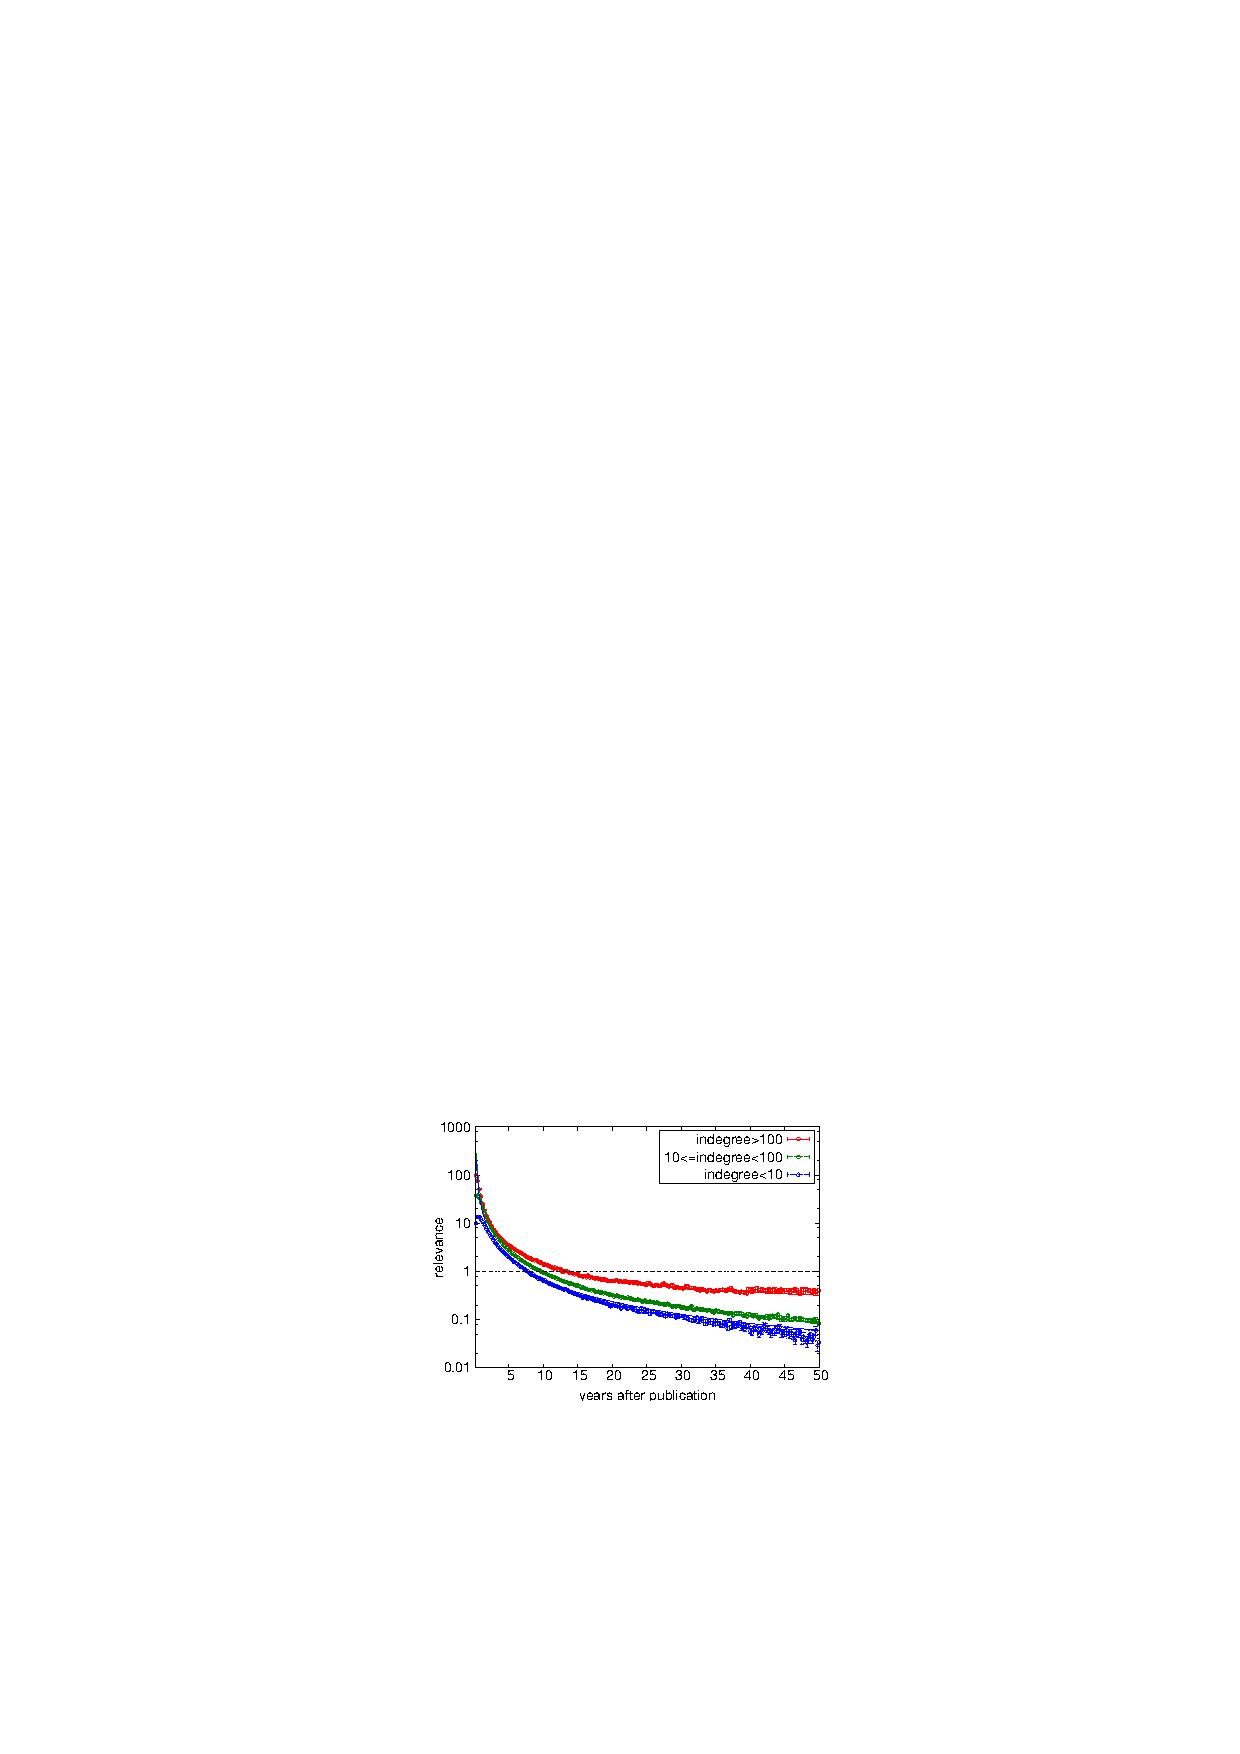
\includegraphics[width=0.7\textwidth]{figures/RelevanceDecayAPS}
        \caption{Temporal decay of the average relevance $r(t)$ of papers in the American Physical Society citation network (1893-2009).
        Papers are clustered in three classes, by their indegree. This behaviour has been formerly highlighted in~\cite{Medo2011}.}
    \end{figure}
\end{frame}

\begin{frame}{How to build a network with the Relevance Model}
    At each discrete time interval $t$, the \textbf{generation algorithm} proceeds as follows:
    \begin{enumerate}
        \item a \alert{new node} is created and connected to an existing node $i$, chosen with probability $\Pi_i^{in}(t)$.
        \item If $t>10$, then $m=10$ existing nodes are sequentially chosen \\ with probability $\Pi_i^{out}(t)$ and become \alert{active}:
        \begin{itemize}
            \item each selected node creates one outgoing link
            \item it selects a node $j$ as a target with probability $\Pi_j^{in}(t)$
        \end{itemize}
    \end{enumerate}
    \vspace{1em}
    \begin{footnotesize}
    \begin{itemize}
        \item No multiple links.
        \item No self loops.
    \end{itemize}
    \end{footnotesize}
\end{frame}

\begin{frame}{Relevance Model:\@ Link generation mechanism}
    When a node $j$ generates a new link at time $t$, the probability that the target is node $i$ is:
    \[
        \Pi_i^{in}(t) \sim (k_i^{in}(t) + 1) \, \eta_i \, f_R (t-\tau_i)
    \]
    \begin{itemize}
        \item $k_i^{in}(t)$: current indegree of node $i$
        \item $\eta_i$: fitness of $i$
        \item $\tau_i$: time at which $i$ enters the network
        \item $f_R$: monotonously decaying function of time
        \item $R_i(t) := \eta_i f_R (t-\tau_i)$: \alert{relevance} of node $i$ at time $t$.
    \end{itemize}
\end{frame}

\begin{frame}{Relevance Model:\@ Active nodes selection}
    In the RM, nodes \alert{continue being active} and generate outgoing links continually.

    Probability of being chosen as an \textbf{active node} at time $t$:
    \[
        \Pi_i^{out}(t) \sim A_i \, f_A (t-\tau_i)
    \]
    \begin{itemize}
        \item $A_i$: activity parameter
        \item $\tau_i$: time at which $i$ enters the network
        \item $f_A$: monotonously decaying function of time
    \end{itemize}
\end{frame}

\begin{frame}{Effects of relevance decay in the RM}
\begin{itemize}
    \item \alert{Slow} or absent relevance decay
    \begin{itemize}
        \item recent nodes receive few links because of preferential attachment
        \item PageRank's bias towards old nodes in scale-free networks
    \end{itemize}
    \item \alert{Fast} relevance decay
    \begin{itemize}
        \item preferential attachment compensated by decay of relevance of old nodes
        \item recent nodes can reach high indegree
        \item recent nodes mostly point to other recent nodes, because of relevance decay of older nodes
        \item old nodes point to nodes of every age because of activity
    \end{itemize}
\end{itemize}
% Figure 1 ?
\end{frame}

\begin{frame}{What makes a ranking algorithm ``good''?}
    \begin{quote}
        A good ranking algorithm is expected to produce \\ an unbiased ranking where both \alert{recent} and \alert{old} nodes \\ have \alert{the same chance to appear at the top}.
    \end{quote}
    \begin{itemize}
        \item In growing networks with temporal effects, \alert{PageRank can fail} to achieve this.
        \item Let's compare PageRank with the elementary \alert{indegree ranking}.
    \end{itemize}
\end{frame}

\begin{frame}{PageRank time bias: numerical simulation of RM}
    \begin{figure}
        \begin{columns}
            \column{0.7\textwidth}
                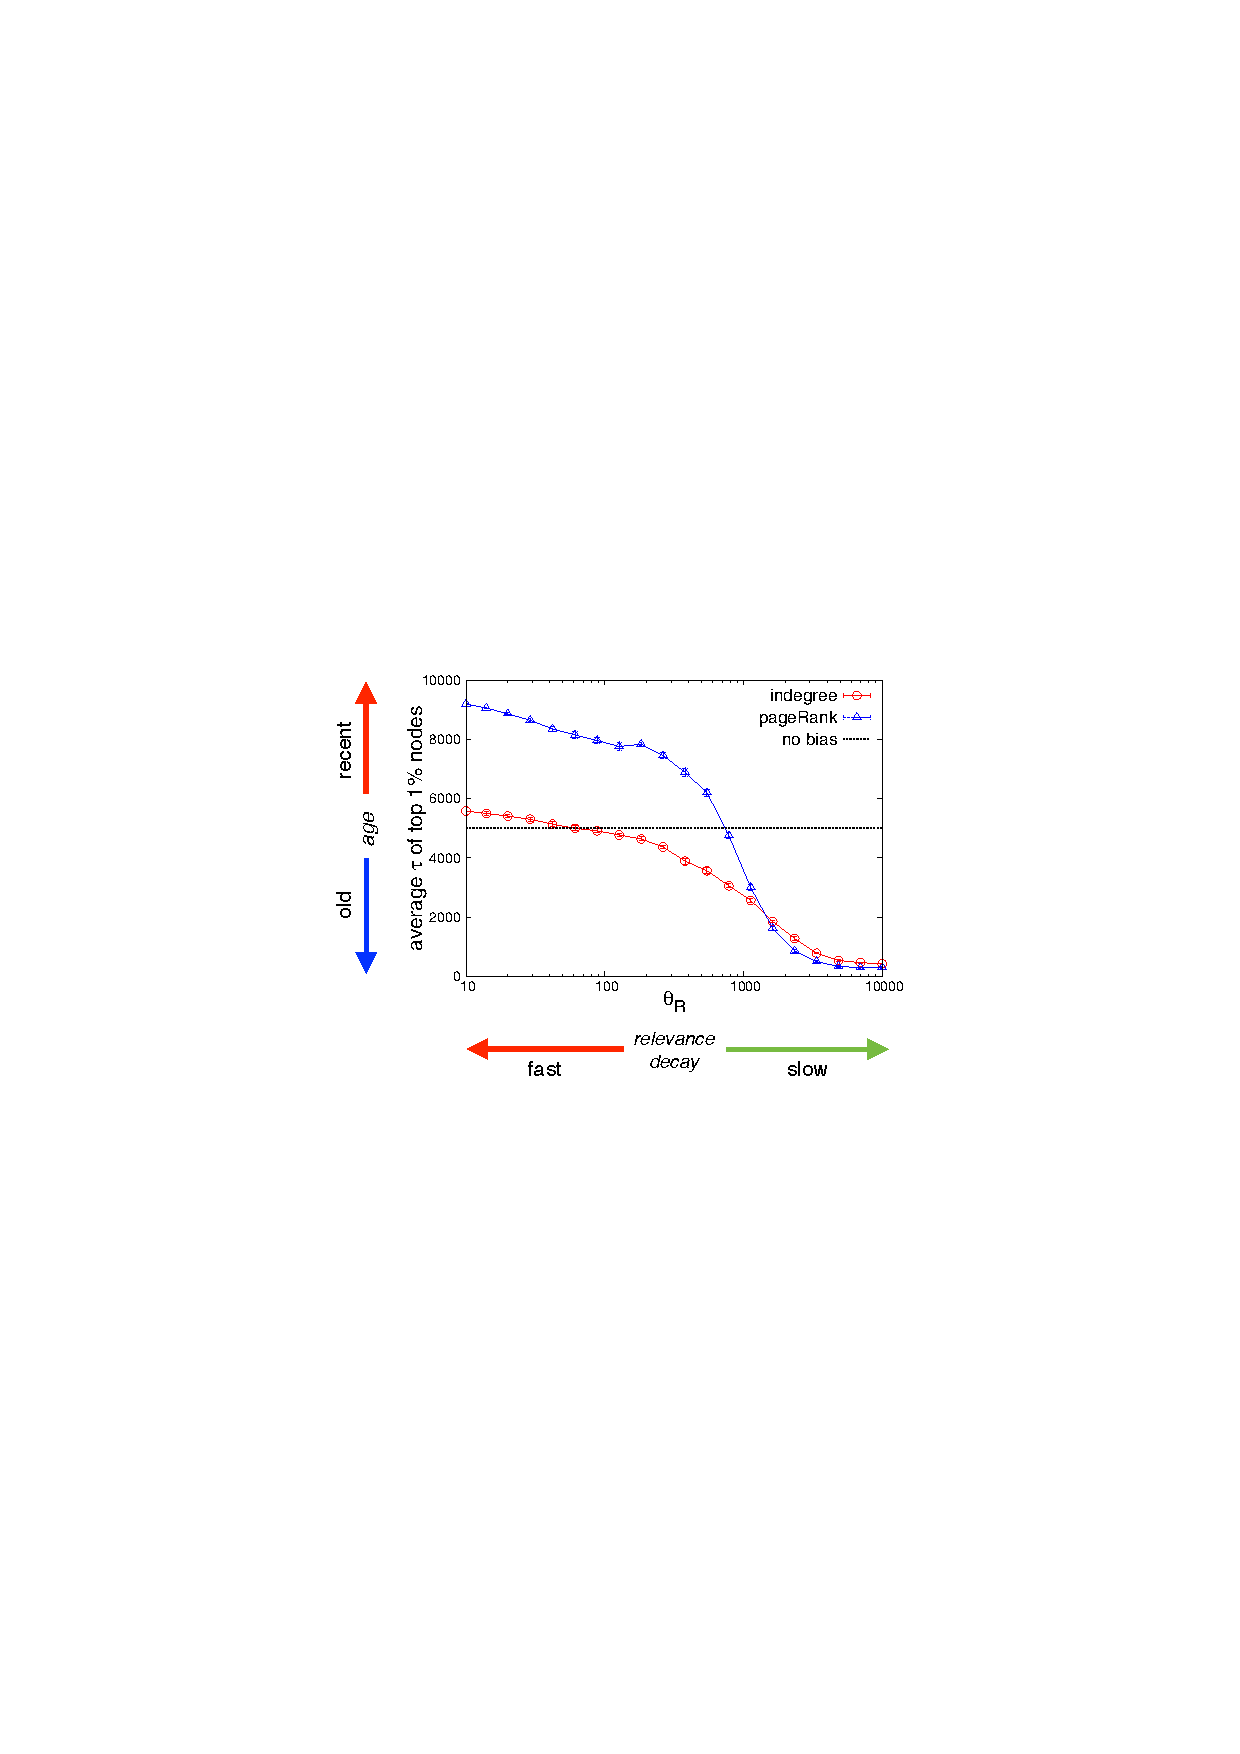
\includegraphics[width=1.0\textwidth]{figures/PageRank_time_bias}
            \column{0.4\textwidth}
                \begin{footnotesize}
                \begin{itemize}
                    \item Relevance decays as $f_R(t) = \exp(-\frac{t}{\theta_R})$.
                    \item Activity decays exponentially, but very slowly ($\theta_A=N$).
                    \item $N=10000$
                \end{itemize}
                \end{footnotesize}
    \end{columns}
    \caption{Average time of entrance of 1\% of nodes of PageRank and indegree rankings, in the RM model.}
    \end{figure}
\end{frame}

\begin{frame}{PageRank vs.\ indegree: correlation with fitness in RM}
    \begin{figure}
        \begin{columns}

        \column{0.6\textwidth}
            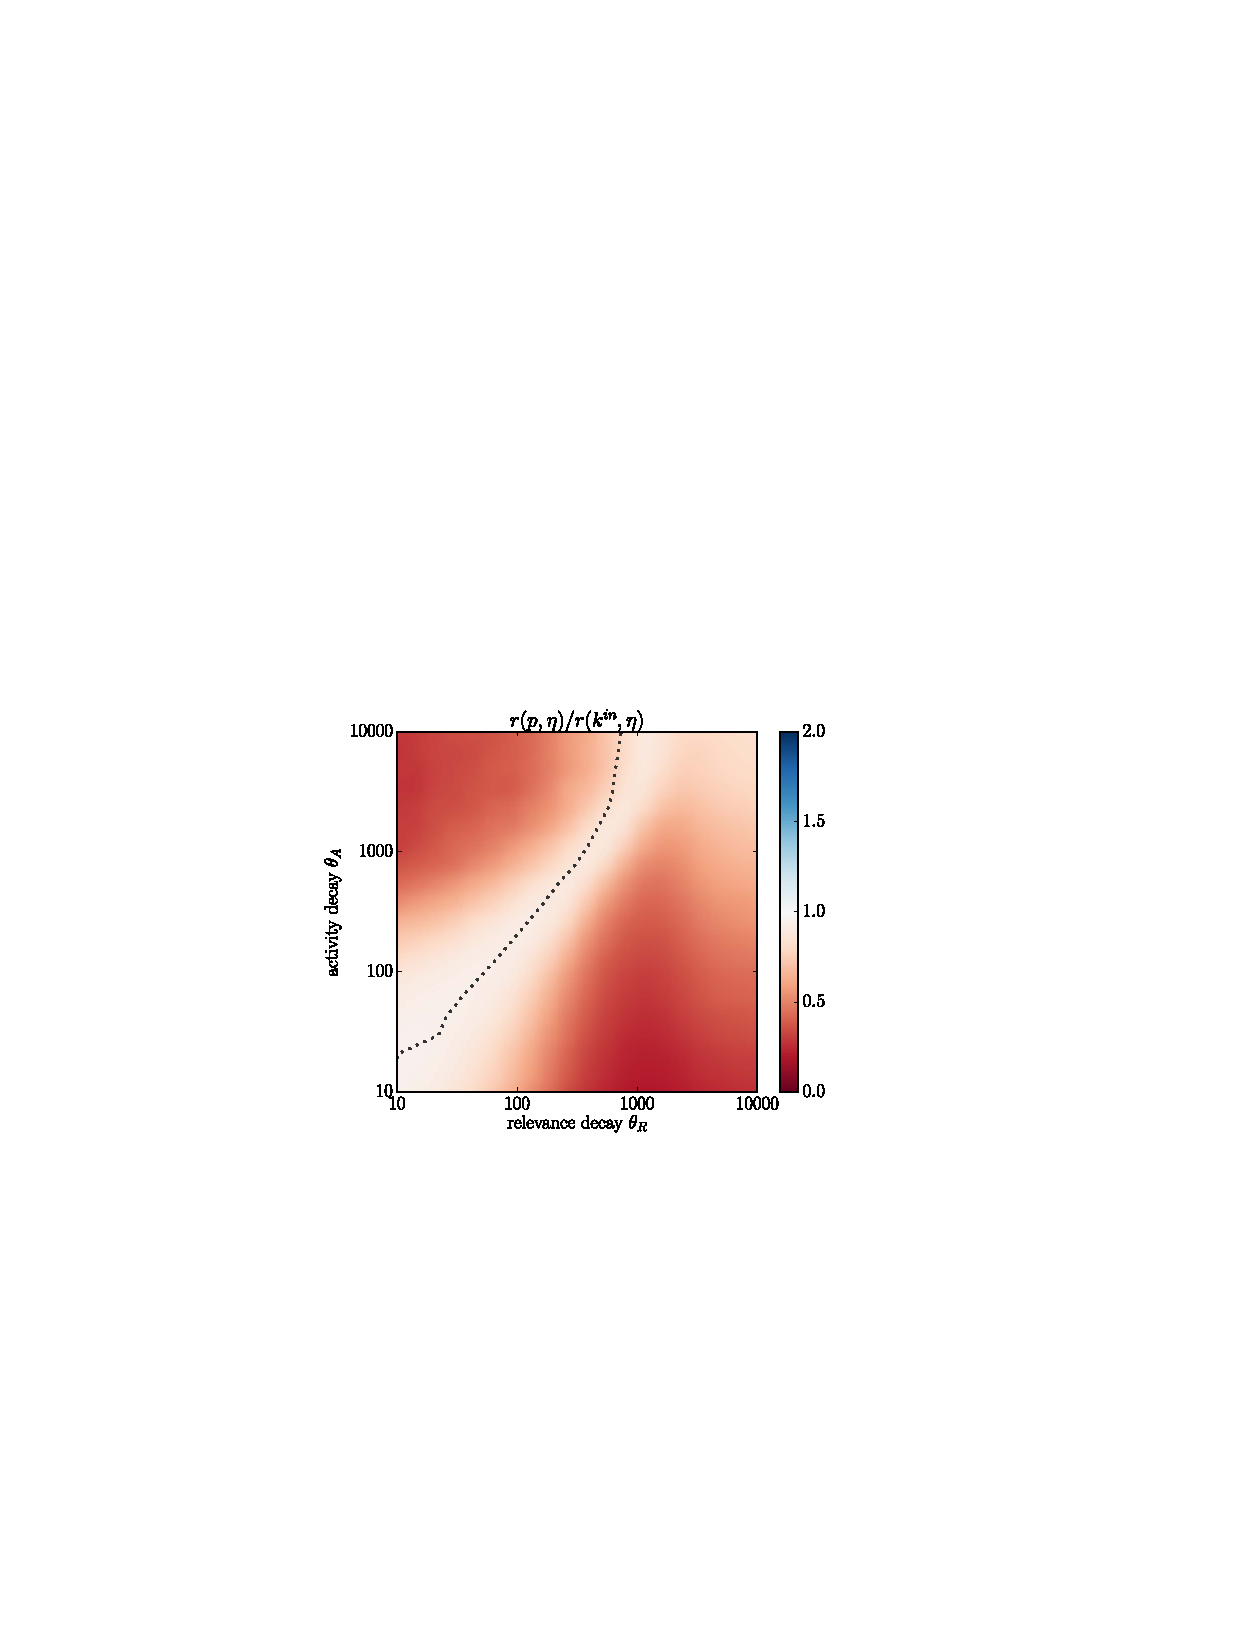
\includegraphics[width=1.0\textwidth]{figures/PageRankRM_heatmap}

        \column{0.4\textwidth}

            \begin{footnotesize}
                \begin{itemize}
                    \item $r(p, \eta)$: correlation PageRank-fitness
                    \item $r(k^{in}, \eta)$: correlation indegree-fitness
                \end{itemize}
            \begin{itemize}
                \item $\rho(\eta) = \exp(-\eta)$
                \item $\rho(A) = 2A^{-3}, \; A \in [1, \infty]$
            \end{itemize}
        \end{footnotesize}
        \end{columns}

    \caption{Comparison of performance of PageRank and indegree (RM data). \newline
    PageRank yields no improvement with respect to indegree. \newline
    Diagonal: no temporal bias towards recent or old nodes.}
\end{figure}
\end{frame}
